% MECH5720 working report, 3 November 2026.
% Adapted from the downloaded iccp26_template.tex by Ayan Chakrabarti,
% modified by Ioannis Gkioulekas, based on Michael Shell's IEEEtran skeleton.
% The supplied IEEEtran.cls is retained unchanged, with its original notices.
% This is a course project draft, not an ICCP/PAMI submission.
\RequirePackage[T1]{fontenc}
\documentclass[10pt,journal,compsoc]{IEEEtran}
\usepackage[nocompress]{cite}
\usepackage{url,amsmath,amssymb,graphicx,booktabs,array,xcolor}
\usepackage[hidelinks]{hyperref}
\newcommand{\pending}[2]{\par\smallskip\begin{samepage}\noindent\textcolor{red!65!black}{\textbf{[PENDING #1]}} \textit{#2}\par\end{samepage}}
\newcommand{\verify}[1]{\textcolor{red!65!black}{\mbox{\textbf{[VERIFY:}} \textbf{#1]}}}
\newcommand{\micros}{\,\mu\mathrm{s}}
\title{Event-Based Structured-Light 3D Scanner:\\Static Reconstruction and Evaluation}
\author{Aryan Rai, Aditya Solanki, Kailas Viswanathan Anilkumar,\\Nadeen Periyasamy, and The Son Le\IEEEcompsocitemizethanks{\IEEEcompsocthanksitem MECH5720, The University of Sydney. Revised working draft, 3 November 2026. Red placeholders identify uncompleted measurements or verification; they are not results.}}
\markboth{MECH5720 Major Project --- Working Draft, 3 November 2026}{}
\begin{document}
\IEEEtitleabstractindextext{%
\begin{abstract}
We built a line-light scanner using a hybrid event/grayscale camera, a positional servo and team-designed mounts. A stationary-pulse fallback produced partial shoe reconstructions with 960 grayscale-derived points and 494 event-derived points across 20 calibrated commands. On 339 common rows from a reserved board pose, equal-command depth root-mean-square errors were 8.42\,mm and 8.07\,mm, respectively. This reference shares the camera model and reported target scale, so it does not establish independent absolute accuracy. A fixed visible-shoe image mask gave sample coverage of 6.85\% for grayscale and 3.49\% for events. Three acquisitions at each of five commands showed position-dependent repeatability, without a consistent winner. One unknown neutral-density filter reduced the measured digital stripe signal to 0.43 times the recent unfiltered mean; residual image displacement prevents treating this as calibrated optical transmission. A static pulse timing audit had prediction residuals up to 47.55\,ms. The prototype demonstrates static reconstruction and quantitative diagnostics, while continuous reconstruction, independent geometry validation and calibrated speed/attenuation curves remain incomplete.
\end{abstract}
\begin{IEEEkeywords}Structured light, event cameras, triangulation, calibration, experimental validation.\end{IEEEkeywords}}
\maketitle

\IEEEraisesectionheading{\section{Introduction}\label{sec:intro}}
\IEEEPARstart{A}{moving} projected line makes surface shape observable through camera--projector triangulation. An event sensor is attractive because stripe transitions can produce temporally local observations, while ordinary frames also sample the background. The proposed research question was whether calibrated depth could be recovered from a smoothly swept weak line, and how error and coverage change with sweep speed and optical attenuation~\cite{pitch}. Those advantages are hypotheses, not consequences of choosing an event camera.

Our completed evidence concerns the proposal's slower \emph{stop-and-pulse fallback}: the servo holds a command, a bounded light pulse is recorded, and both grayscale and event candidates are intersected with a fixed calibrated plane. We demonstrate real partial surface profiles, reserved-board errors, repeatability and image-space coverage. We also report a limited filter experiment and a timing failure rather than substituting illustrations for measurements. Continuous moving-stripe reconstruction and several independent-reference tests remain pending.

\subsection{Contribution beyond the laboratories}
The team designed and built a base, camera and servo mounts, rotating projector cradle and object pedestal, then integrated a DAVIS240C, feedback controller and acquisition software (Fig.~\ref{fig:rig}). This adds active geometric depth measurement and actuator integration to the lab kit. Lab~1 studied classical imaging trade-offs; Lab~2 reconstructed illumination components for relighting; Lab~3 measured coded-aperture point-spread functions and deconvolution; and Lab~4 calibrated a diffuser-based lensless system~\cite{lab1,lab2,lab3,lab4}. Our addition is the team-built electromechanical triangulation system, beyond the lab and bonus tasks. Fixed settings, calibration, baselines and retained failures follow the laboratory reporting approach.

\begin{figure}[!t]\centering
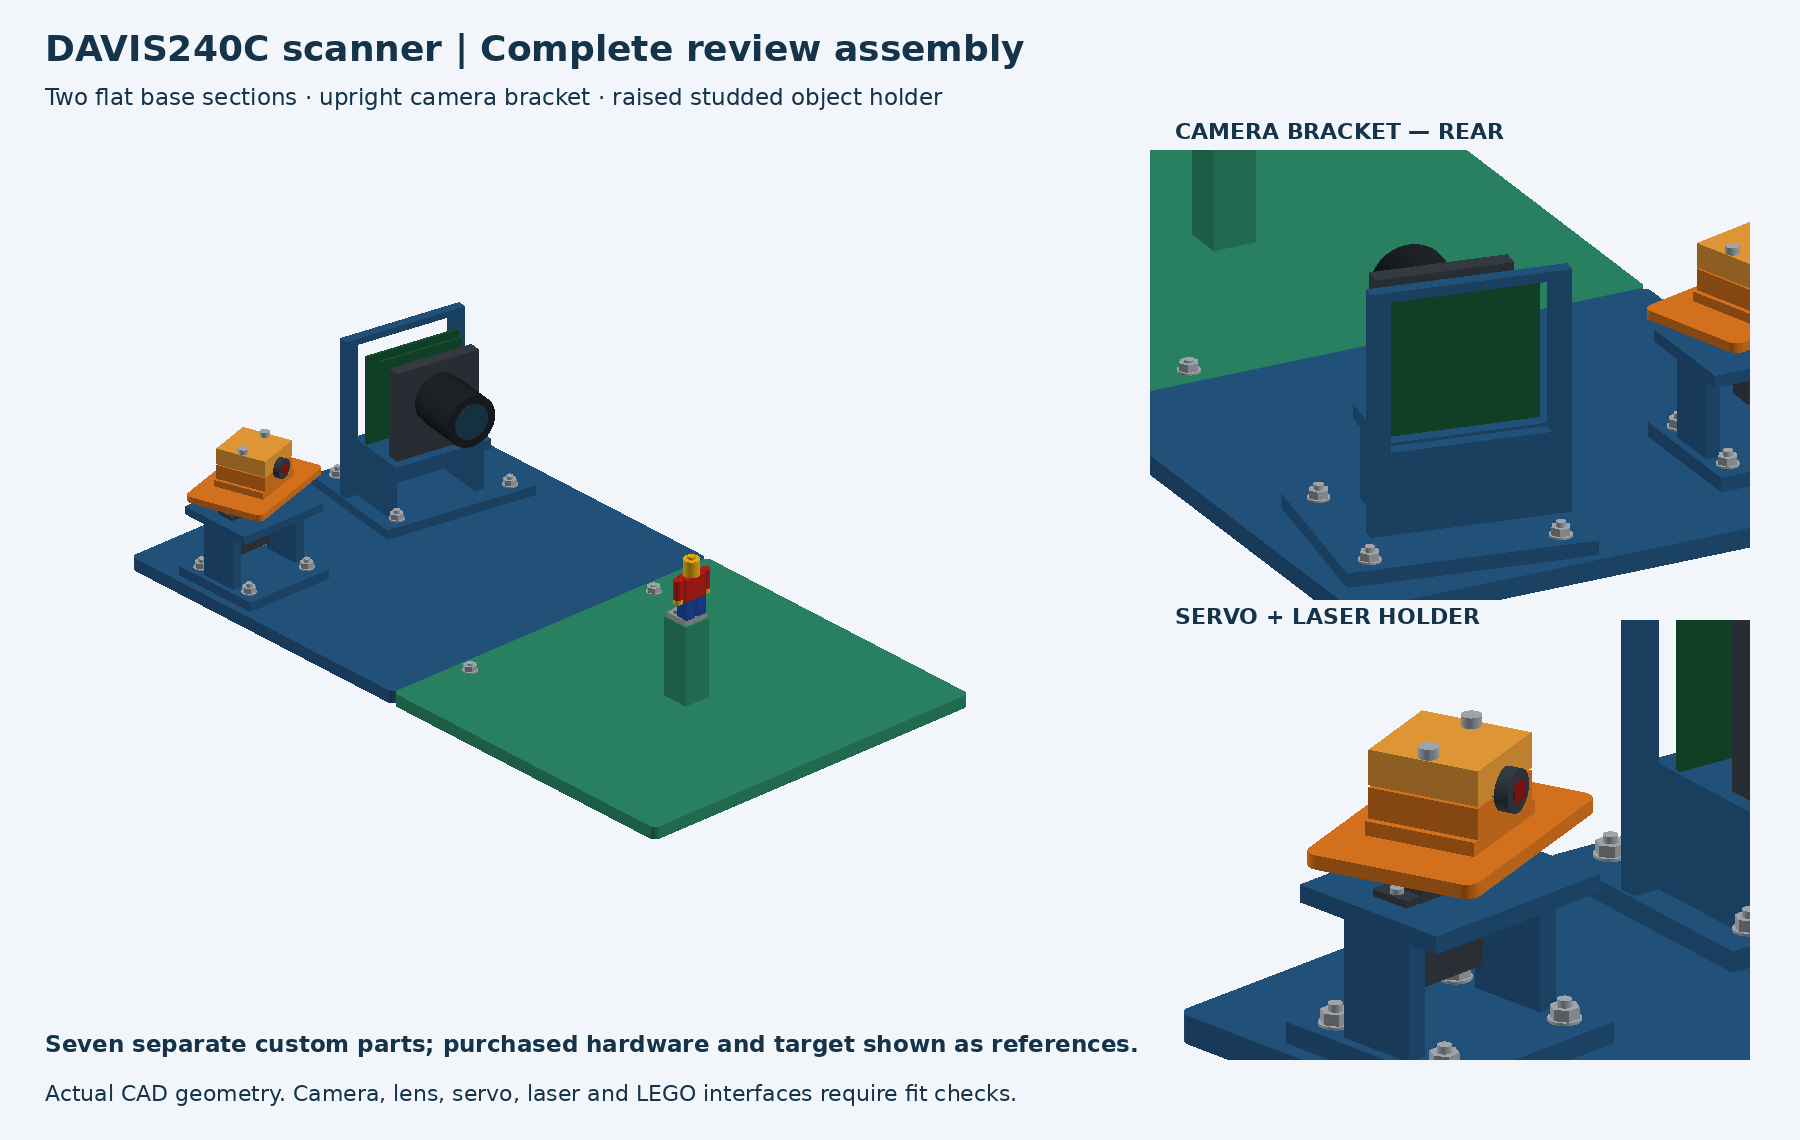
\includegraphics[width=.46\columnwidth,height=1.3in,keepaspectratio]{figures/scanner_cad_review.png}\hfill
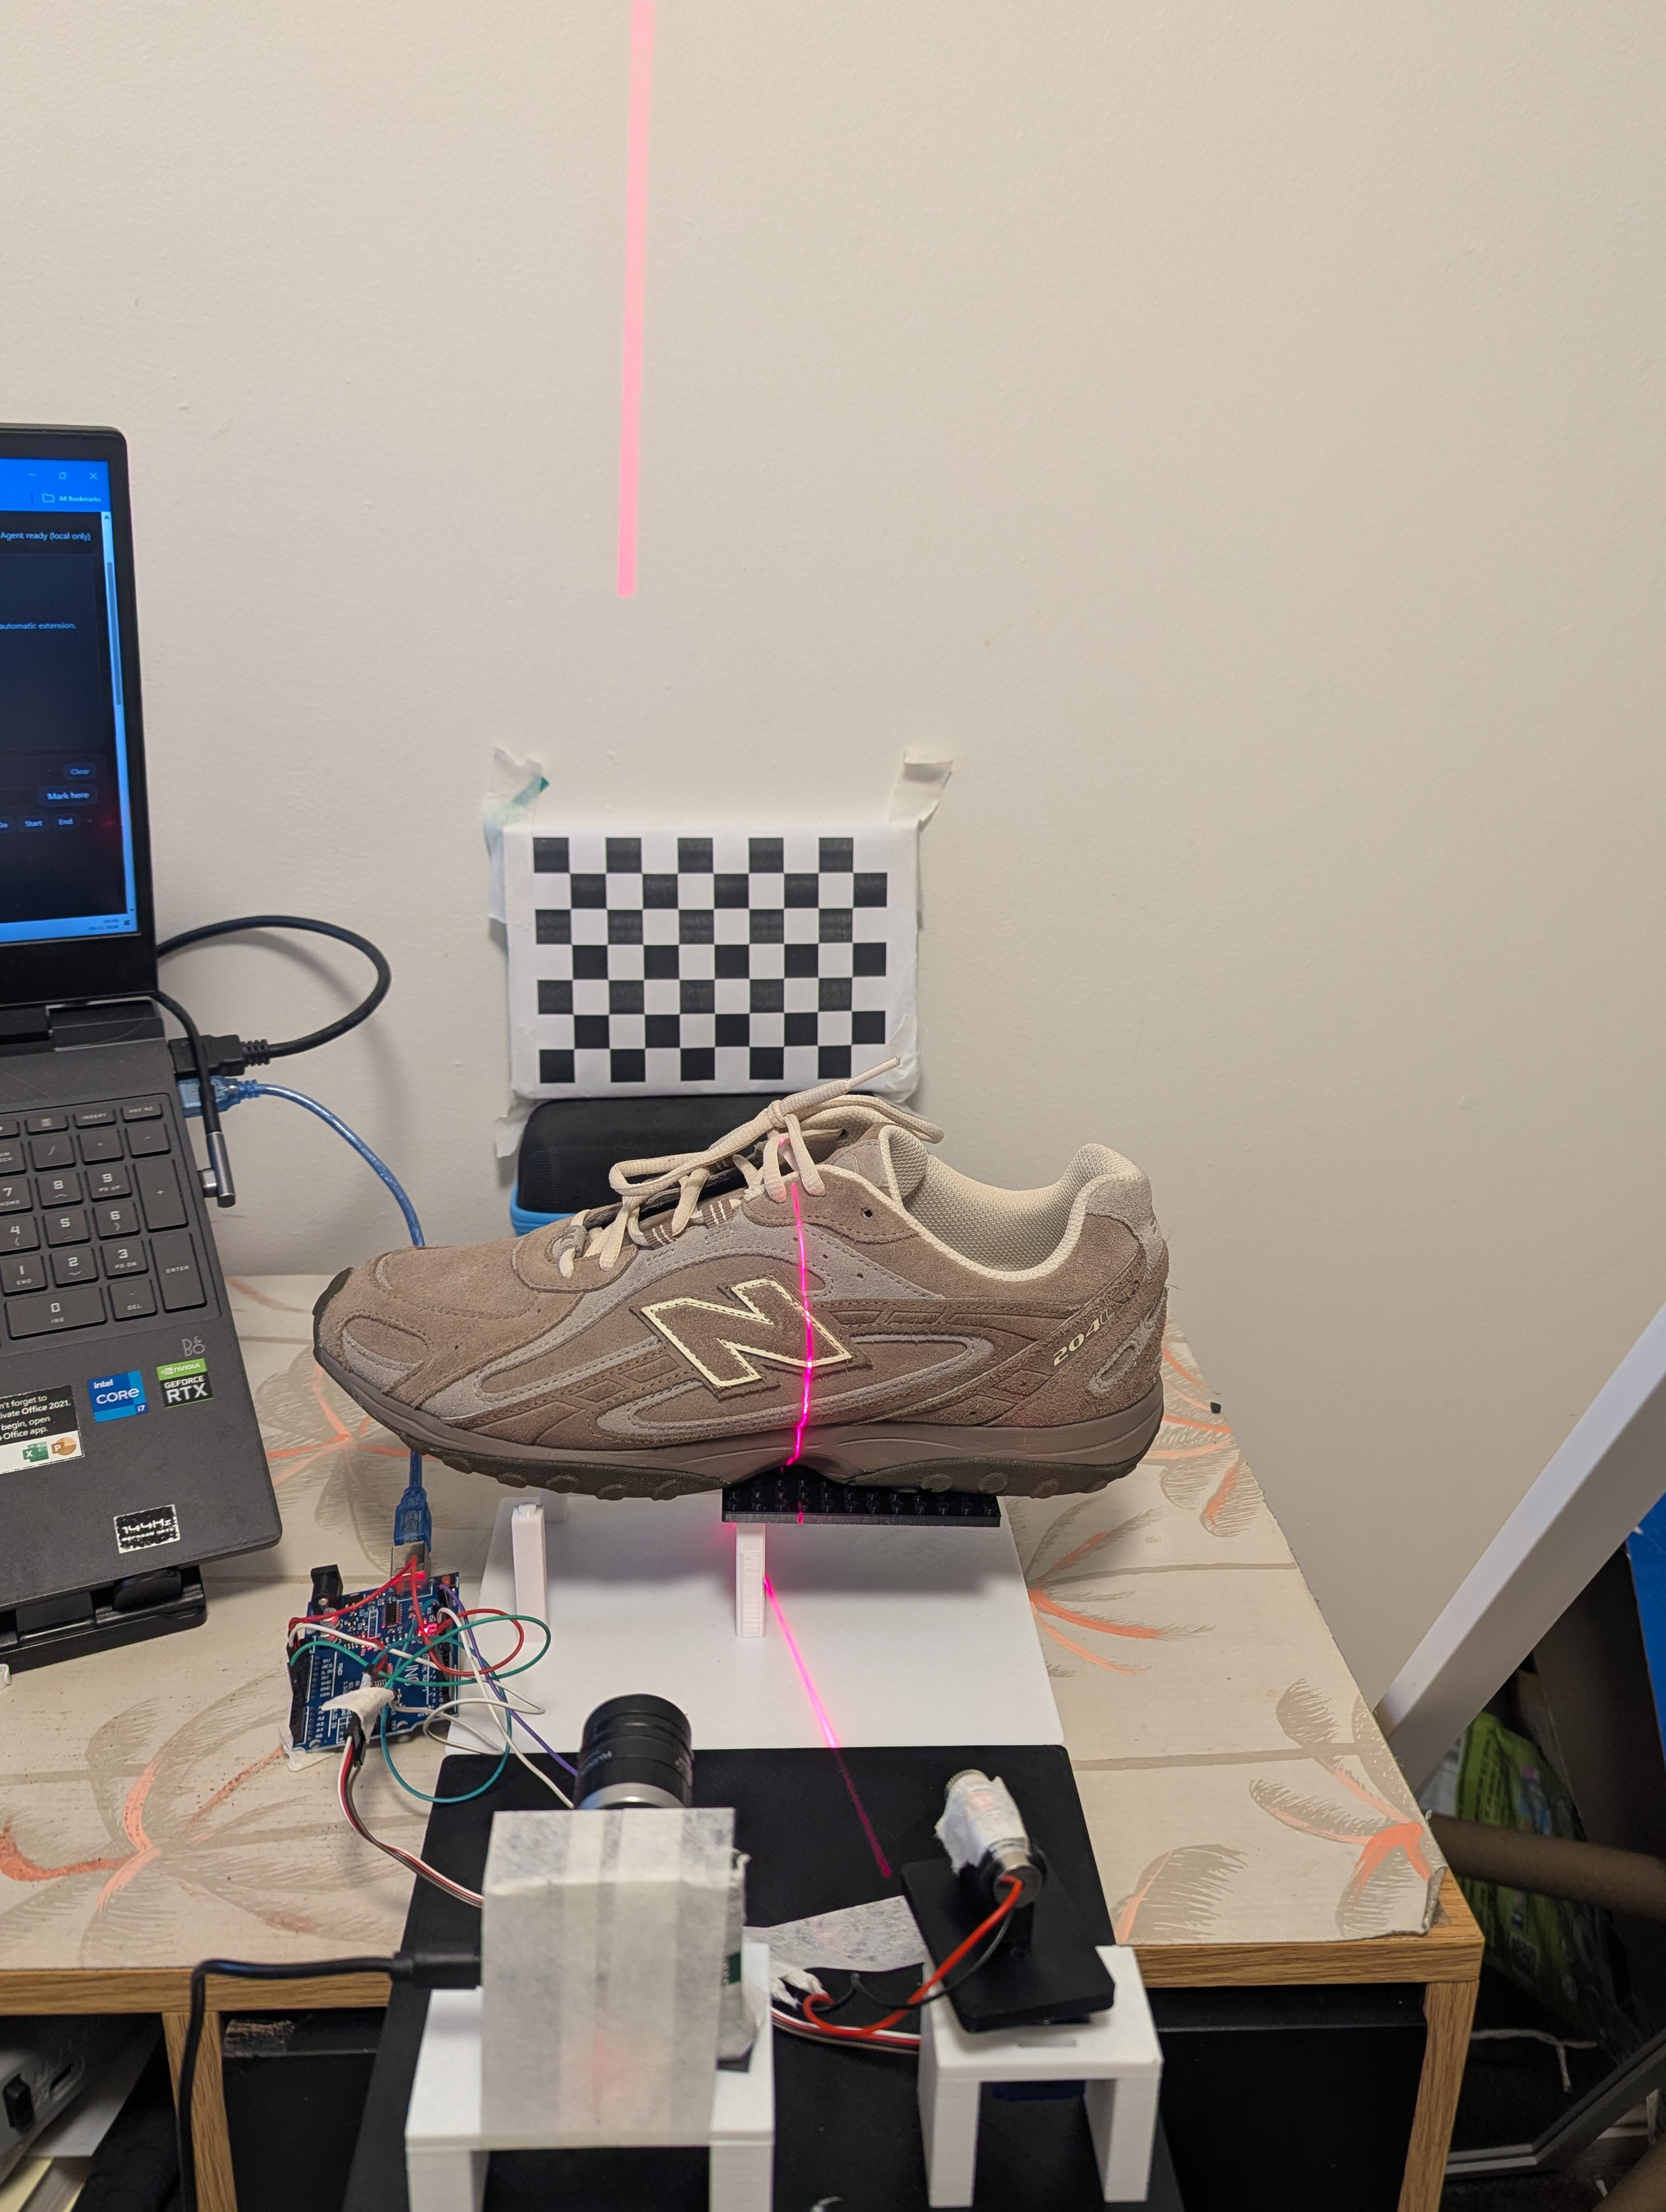
\includegraphics[width=.27\columnwidth,height=1.3in,keepaspectratio]{figures/real_stripe_photo.jpg}\hfill
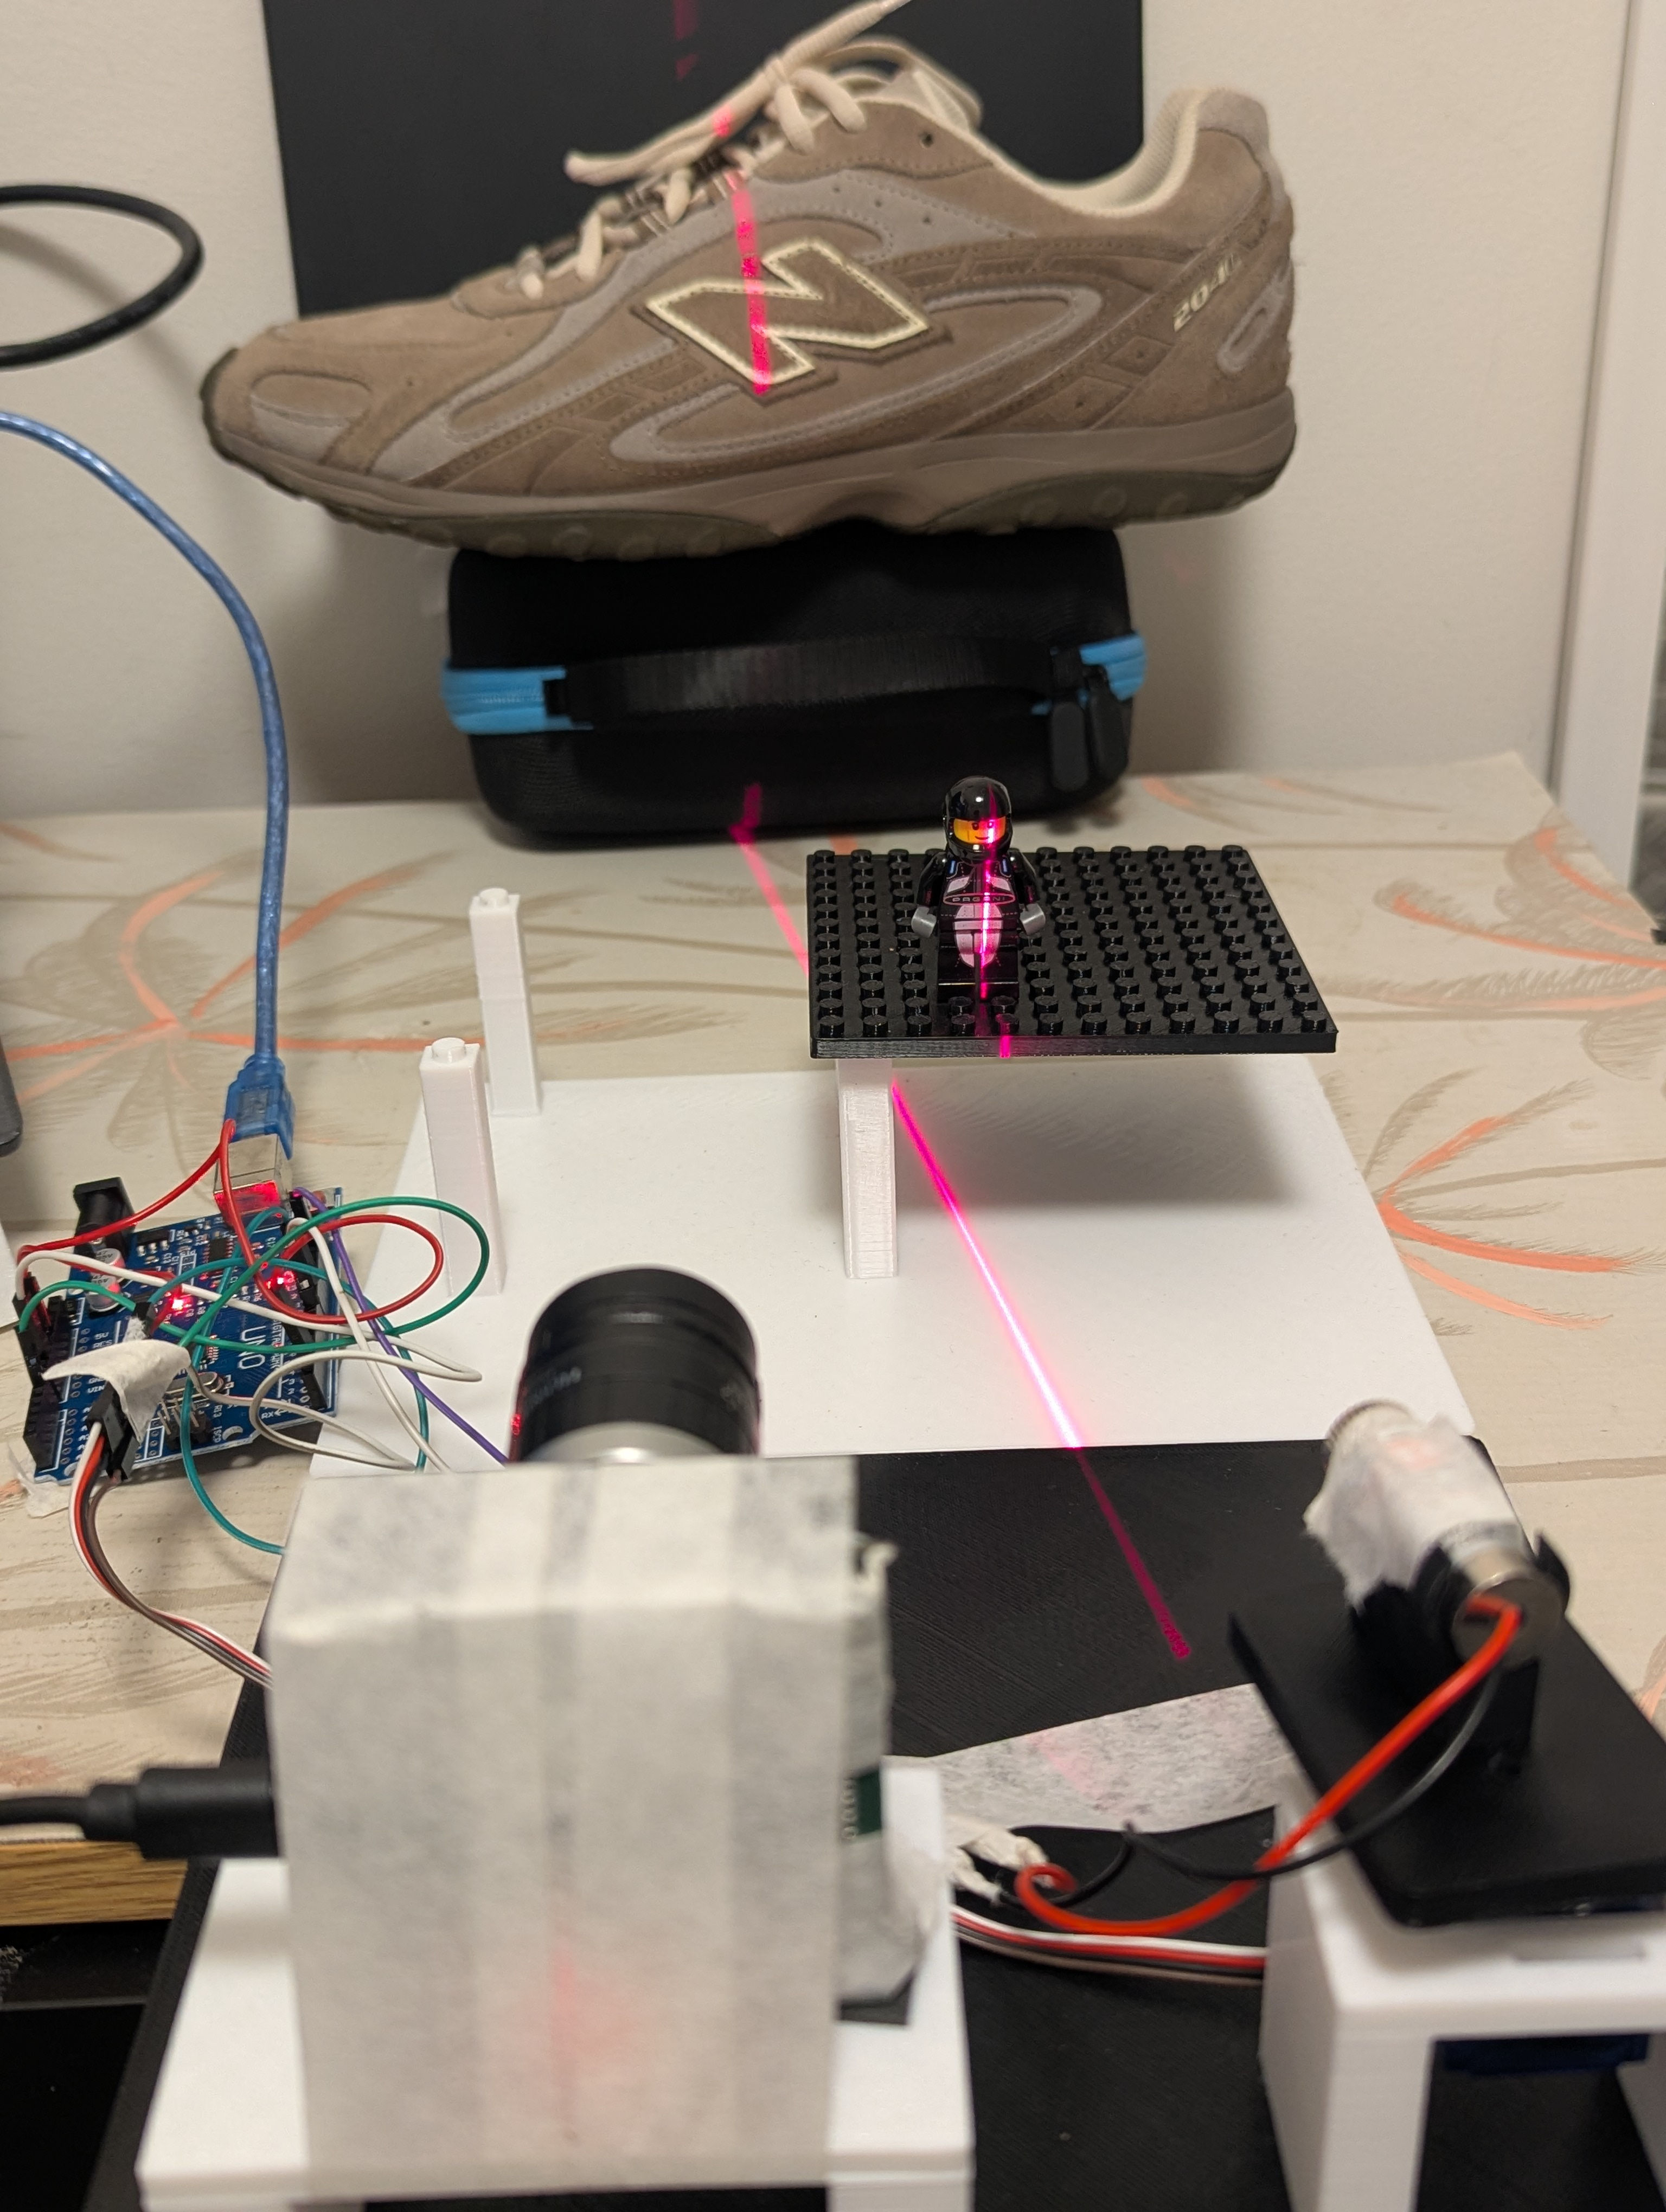
\includegraphics[width=.22\columnwidth,height=1.3in,keepaspectratio]{figures/assembled_rig.jpg}
\caption{CAD review (left), real projected stripe on the shoe (centre) and assembled rig (right). CAD is the intended design with representative purchased parts, not measured as-built geometry; photographs document the implementation. Beam visibility is not depth accuracy.}\label{fig:rig}\end{figure}

\section{Related Work}
MC3D combines motion-contrast sensing with scanned illumination to exploit sparse temporal measurements~\cite{matsuda2015}. It motivates our scanner, but its reported capabilities cannot be transferred to our servo implementation. ESL uses spatio-temporal consistency to address event matching and timing effects in a raster-scanned projector system~\cite{muglikar2021}; we do not implement its optimisation or claim equivalent performance. The event-vision survey of Gallego \emph{et al.}~\cite{gallego2022} provides the broader sensor/algorithm context. Our camera calibration follows the planar-target approach associated with Zhang~\cite{zhang2000}, followed by a documented corner-detection audit. The project contribution is a course-scale physical implementation and evaluation, not novelty over these papers.

\section{System and Reconstruction Method}\label{sec:method}
\subsection{Physical and software implementation}
The DAVIS240C provides native $240\times180$ grayscale active-pixel-sensor (APS) frames, events and an inertial stream. A positional feedback servo rotates the line projector. An Uno-compatible controller runs firmware~v1.7; a single Chrome dashboard owns its serial connection, while one persistent camera service owns the DAVIS. Command-line clients submit uniquely identified operations and retain native recordings, sidecars, controller messages and feedback samples. An uncertain operation is inspected rather than automatically replayed.

The implemented observation protocol holds the current command for 3\,s in darkness, emits for 1\,s, records 0.5\,s after extinction, and ends off/disarmed with the servo released. Native camera recordings span 12\,s, including setup margins. Feedback variation is advisory in observation mode; a completed trace is not proof of a settled optical plane. Host controls are not safety-rated, and no feedback-to-degree conversion is assumed.

The reported build substitutes an R3-type controller and D7-supplied eBay line module for the proposed R4/transistor/Class~1 specification. Installed labels and controls are not independently verified. \verify{module/servo/lens, driver/wiring, supply, controls, as-built dimensions and optics configuration}. Nominal CAD baseline and target distance are not physical ground truth.

\begin{figure}[!t]\centering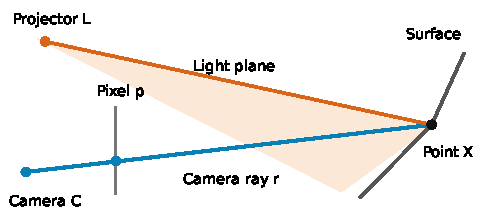
\includegraphics[width=\columnwidth]{figures/triangulation_compact.pdf}
\caption{Conceptual triangulation section (not to scale), not a rig photograph or measurement. The undistorted camera ray through pixel $\mathbf p$ intersects a calibrated light plane at $\mathbf X$. The current implementation uses held commands; the diagram does not establish continuous timing.}\label{fig:geometry}\end{figure}

\subsection{Camera rays and static light planes}
Let $\mathbf p=(x,y)$ be a retained stripe centre. Undistortion using the camera matrix $K$ and distortion parameters $D$ gives ray $\mathbf r=(x_n,y_n,1)^\mathsf T$. For a calibrated static command $u$, the plane and ray meet as illustrated in Fig.~\ref{fig:geometry}:
\begin{equation}
 \mathbf n_u^\mathsf T\mathbf X+d_u=0,\qquad
 \mathbf X=-\frac{d_u}{\mathbf n_u^\mathsf T\mathbf r}\mathbf r.
 \label{eq:intersection}
\end{equation}
We reject near-parallel, nonfinite or nonpositive-depth intersections. Distances inherit the target's reported millimetre scale. Here $u$ indexes a PWM command, not measured shaft angle. Continuous operation would require a validated camera-time-to-feedback/plane mapping, which is not supplied by matching timestamp ranges.

The intrinsic candidate uses a reported $9\times6$ inner-corner target with 18\,mm square pitch. A 60\,s recording contains 821 APS frames. A board-region quality audit avoided rejecting valid views merely because black squares/background occupied a large image fraction. Twenty-five candidate views were re-detected consistently with a sector-based detector at $4\times$ resolution and cross-checked at $2\times$. Three training candidates were excluded for cross-scale disagreement or grid anomalies; original data and reasons were retained. Seventeen training views and the same five reserved views were used for the final audit. Reserved views had already been inspected during diagnosis, so they are not an untouched test set.

For light-plane calibration, detected stripe rays intersect each posed board to produce 3D lines. Multiple lines at one command define a plane. Poses A--C fit the model; D is excluded and used for validation (Fig.~\ref{fig:poses}). Twenty planes from 1569 to $1647\micros$ were fitted: 18 use three board poses and two use two. The insufficiently supported $1651\micros$ command is absent. The model was frozen before D evaluation and hash-checked afterwards. No D alignment, refit or bias correction was applied.

\begin{figure}[!t]\centering
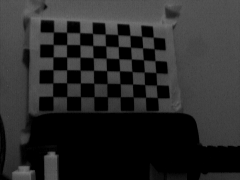
\includegraphics[width=.48\columnwidth]{figures/pose_A.png}\hfill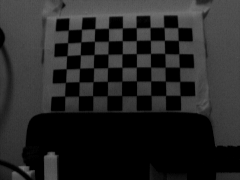
\includegraphics[width=.48\columnwidth]{figures/pose_B.png}\\[-2pt]
{\footnotesize A: fitting tilt\hspace{.55in}B: opposite fitting tilt}\\
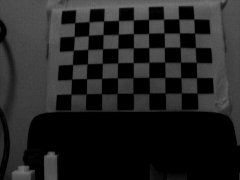
\includegraphics[width=.48\columnwidth]{figures/pose_C.png}\hfill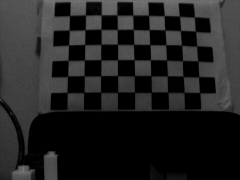
\includegraphics[width=.48\columnwidth]{figures/pose_D.png}\\[-2pt]
{\footnotesize C: closer fitting pose\hspace{.35in}D: reserved test}
\caption{Actual DAVIS board reference images. The board scale is user-reported; pitch, print distortion and flatness were not independently verified.}\label{fig:poses}\end{figure}

\subsection{APS and event stripe candidates}
The APS detector subtracts the first three-frame median, selects frames whose global positive-change signal exceeds half its peak, and retains at least five lit frames. On rows 20--105, candidate pixels require change $>20$ and intensity $>40$ digital levels. Contiguous row groups must be 1--12 pixels wide. The strongest group is rejected if a runner-up exceeds 0.67 of its energy or any selected pixel is $\ge250$. A row median is retained when supported in at least half the selected lit frames.

The event detector uses no APS spatial stripe mask. In the same fixed image rows, 25\,ms polarity-count peaks separated by the known 1\,s pulse duration select candidate ON/OFF transitions. Primary windows are 50\,ms per transition; 20 and 100\,ms are sensitivity settings. Pixels require at least three events and background-subtracted count at least two; the same group-width/ambiguity screens are applied. ON and OFF row centres must agree within 3 pixels. This corroboration is a heuristic, not confirmed laser identity. Parameters were developed on saved shoe data, then applied unchanged to reserved-board and fresh repeat recordings. There is no untouched, manually labelled detector benchmark.

Both methods use the same native recordings, camera model and fixed planes. APS pools selected 35\,ms lit frames, whereas events use two 50\,ms windows. Thus the comparison is matched in scene/geometry but not in temporal integration, photon budget or acquisition speed. Event accumulation images are never substituted for the APS baseline.

\begin{figure*}[!t]\centering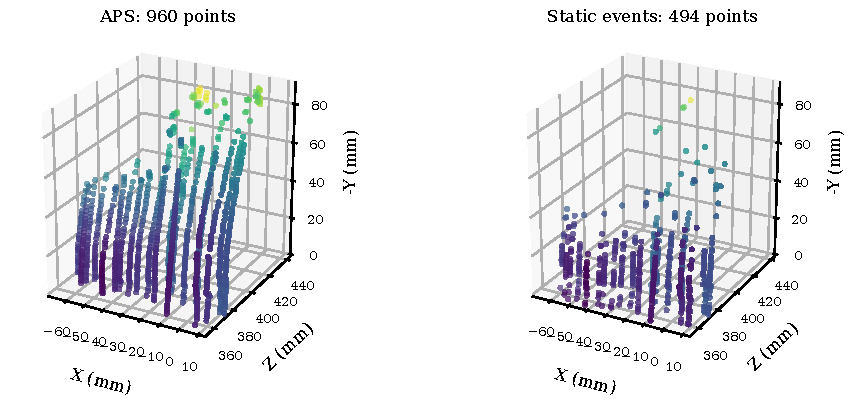
\includegraphics[width=.90\textwidth]{figures/paired_clouds.pdf}
\caption{Actual retained partial shoe point clouds on equal coordinate axes. Camera-coordinate millimetres inherit the reported target scale. No interpolated plane, surface mesh, test alignment or independent shoe accuracy is claimed.}\label{fig:clouds}\end{figure*}

\section{Experimental Design and Metrics}\label{sec:metrics}
\subsection{Depth, agreement and repeated acquisitions}
For the D board, an observation's ray intersects the posed reference board to give $Z_{\mathrm{ref}}$. Depth residuals are $e=Z_{\mathrm{pred}}-Z_{\mathrm{ref}}$. We report per-command RMS and equal-command aggregation,
\begin{equation}
 E=\sqrt{\frac1{M}\sum_{u=1}^{M}\frac1{N_u}\sum_i e_{ui}^{2}}.
\end{equation}
The event/APS comparison uses only common command/row pairs inside the known inner-corner rectangle. This prevents a method's extra rows changing the comparison denominator, but may favour easy detections. The board reference shares $K$ and the reported target scale; it is not independent absolute ground truth. Shoe event--APS depth disagreement likewise measures agreement, not accuracy.

A later shoe placement defines a separate repeatability condition. Three acquisitions at each of five fitted commands were evaluated without alignment. For rows present in both methods and all three trials, precision is
\begin{equation}
 S_u=\sqrt{\frac1{|R_u|}\sum_{y\in R_u}\frac1{n-1}
 \sum_{j=1}^{n}(Z_{uyj}-\bar Z_{uy})^2},\quad n=3.
\end{equation}
The independent units are acquisitions, not rows/events. An image row identifies a sampling ray, not an independently tracked material point. $S_u$ combines mechanical, detector and scene variability; common-row selection can suppress failures, so support counts are also retained.

\subsection{Fixed-denominator image-space coverage}
A manually outlined visible-shoe-body mask $\Omega$ in a laser-off photo contains 13,715 native pixels. It excludes background, pedestal and loose laces above the main body. Retained centres are rounded to native bins and deduplicated. With occupied set $B$, coverage is
\begin{equation}
 C_{\mathrm{image}}=100\,|B\cap\Omega|/|\Omega|.
\end{equation}
The same mask is used for both methods. It is approximate and post-acquisition; one-/two-pixel boundary perturbations are sensitivity checks, not confidence intervals. Full-body coverage retains regions outside the processed rows to expose missing sampling. This metric is image-space sample occupancy, not physical 3D surface-area completeness or accuracy. No gap filling or mesh is counted as measurement.

\begin{figure*}[!t]\centering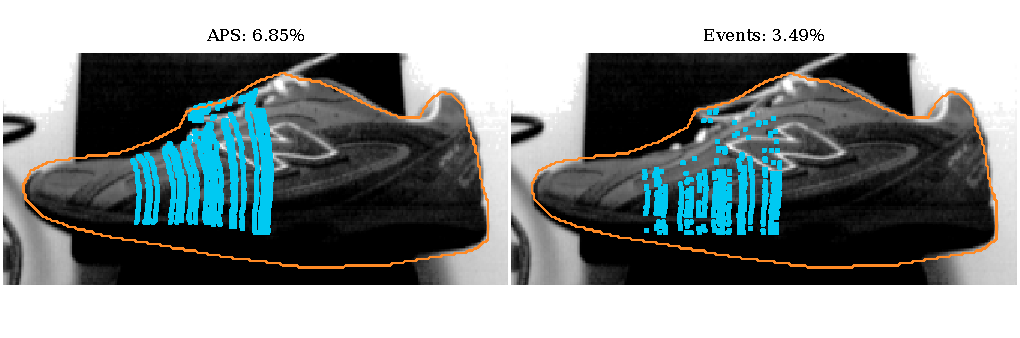
\includegraphics[width=.90\textwidth]{figures/coverage_compact.pdf}
\caption{Same fixed visible-body outline for both outputs. Cyan bins show retained samples, not filled surface. The denominator includes the toe, heel and lower body even where no profiles were reconstructed.}\label{fig:coverage}\end{figure*}

\subsection{Filter and optical timing diagnostics}
The ND retry uses two recent unfiltered controls and three reinserted-filter captures at $1626\micros$, with fixed 35\,ms exposure and 1\,s pulses. A fixed unfiltered-derived stripe neighbourhood measures background-subtracted digital signal. The filter marking, optical transmission and camera radiometric response are unknown. Residual displacement and unequal detector integration prevent a calibrated attenuation interpretation. Earlier insertion/removal attempts are preserved separately rather than pooled.

For timing, an affine relation was fitted to five first-pass ON markers from static pulses. Ten subsequent ON and all 15 OFF markers were reserved for prediction. Event burst peak/median selection is compared with firmware electrical markers. Residuals include optical/polarity response and selection effects as well as clock-model error; they are not isolated hardware latency or absolute timing uncertainty. Resets invalidate this session-specific mapping.

\section{Results and Analysis}\label{sec:results}
\subsection{Camera and reserved-board calibration}
The refined camera fit gives training RMS 0.2351 pixels; five reserved per-view RMS values range from 0.1990 to 0.2965 pixels. The matrix is
\begin{equation}
 K=\begin{bmatrix}307.0201&0&115.7638\\0&306.8715&104.0087\\0&0&1\end{bmatrix}.
\end{equation}
The five distortion coefficients are approximately $(-0.28245,\,0.55350,\,0.003641,\,0.001042,\,-0.89863)$. Leave-one-training-view-out focal ranges are 305.90--307.60 and 305.68--307.43 pixels. Fixing $k_3=0$ gives nearly identical training RMS 0.23515 pixels. Figure~\ref{fig:intrinsic} shows the detector audit. These are sensitivity observations, not confidence intervals or independent depth validation.

The original APS-only reserved-D evaluation gives equal-command RMS 8.63\,mm across 20 commands, with per-command RMS 0.88--17.03\,mm. Restricting both methods to 339 common rows across 19 commands gives 8.42\,mm for APS and 8.07\,mm for events (Fig.~\ref{fig:board}). One command lacks common retained rows. The different denominator explains why the APS value differs from 8.63\,mm; it is not an improved calibration. Position-dependent errors dominate any small aggregate difference, and no event advantage is established.

\begin{figure}[!t]\centering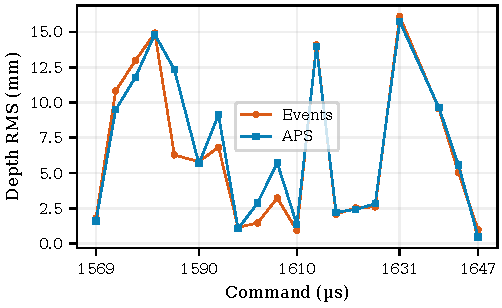
\includegraphics[width=\columnwidth]{figures/board_compact.pdf}
\caption{Reserved D depth RMS on identical command/row support. Shared camera model and reported scale; one board pose, no test alignment. Missing common support is not assigned zero error.}\label{fig:board}\end{figure}

\begin{figure}[!t]\centering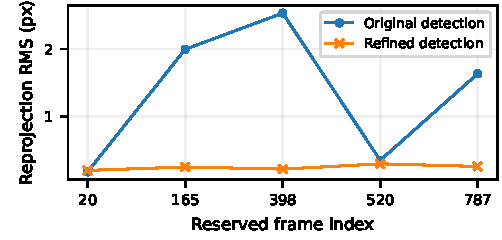
\includegraphics[width=\columnwidth]{figures/intrinsic_refinement_compact.pdf}
\caption{Corner-refinement audit on the same five reserved views. Each model estimates the reserved poses with its intrinsics fixed; reserved views were previously inspected. Training exclusions differ between models. Reprojection errors are pixels, not independent depth accuracy.}\label{fig:intrinsic}\end{figure}

\subsection{Partial shoe reconstruction and sampling}
Twenty fitted positions yield 960 APS points and 494 event points at the primary window (Fig.~\ref{fig:clouds}). On 455 shared shoe rows, horizontal disagreement is 0.3385 pixels RMS and depth disagreement 1.6497\,mm RMS. Both outputs share calibration errors, so close agreement does not prove object accuracy. Event windows 20/50/100\,ms retain 359/494/532 points. All three settings retain zero corroborated candidates in 3,440 sampled laser-off command/row opportunities. These are internal temporal controls, not a labelled false-positive rate.



Of the 960 APS centres, 955 lie in the fixed body outline and occupy 939 unique bins. All 494 event centres lie inside, occupying 478 bins. Full-body image coverage is therefore 6.85\% and 3.49\%, respectively (Fig.~\ref{fig:coverage}). Restricting the denominator to the common processing rows gives 939/11,762$=7.98\%$ and 478/11,762$=4.06\%$. One-pixel erosion/dilation changes full-body APS coverage to 7.06/6.64\% and event coverage to 3.62/3.36\%. This is a sparse partial scan, not full-shoe reconstruction. Coverage counts candidate locations and cannot verify their identity or physical surface accuracy.



The original sparse scan retained 379 points at five positions with 10\,ms APS exposure. A later 3\,ms scan gave 1,929 points at 21 positions using interpolated intermediate planes; retaining only its four directly fitted positions gives 359 points. These are different recordings, not conflicting exposure labels (Table~\ref{tab:history}). Exposure, distance, model and crop changed; point counts do not establish improved accuracy. In the 960-point result, 933 estimated depths lie within command-specific training stripe-depth ranges. This 97.2\% range membership is not accuracy or completeness.

\begin{table}[!t]\caption{Distinct historical shoe datasets. Exposure is per APS frame, not scan duration. Counts are retained points, not independent repeats.}\label{tab:history}\centering
\begin{tabular}{lrrr}\toprule Dataset&Positions&Points&APS (ms)\\\midrule
Original sparse&5&379&10\\
Later fitted subset&4&359&3\\
Later interpolated preview&21&1,929&3\\
Current fitted scan&20&960&35\\\bottomrule\end{tabular}\end{table}

\subsection{Five-line recording for the presentation}
A separate demonstration on 3 November recorded five stationary pulses at 1569, 1590, 1602, 1626 and $1647\micros$, with the ND removed and 35\,ms APS exposure. Five complete 12\,s native recordings contain 821 APS frames and 284,490 events. This is one acquisition per position, not five repeats of one condition. Feedback screens warned at 1602 and $1647\micros$; all operations ended off/disarmed with servo release. These data do not replace the earlier repeatability study or establish new depth after filter handling.

\begin{figure}[!t]\centering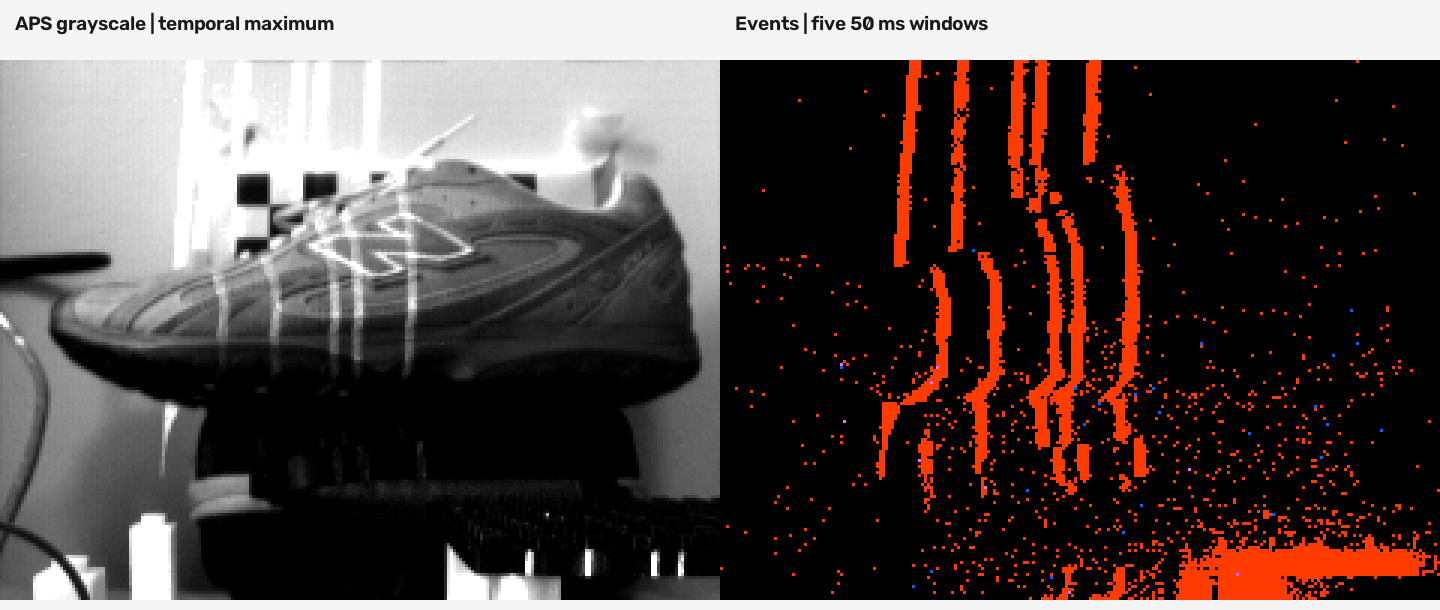
\includegraphics[width=\columnwidth]{figures/five_line_demonstration.png}
\caption{New presentation demonstration: APS (left) and raw polarity events (right). Both are five-position temporal composites, not simultaneous five-line images. Each event picture spans 50\,ms about an automatically selected candidate ON transition; APS frames use 35\,ms exposure within the candidate pulse. Red/blue indicate positive/negative events, including background activity. No new depth or detector-accuracy claim is made.}\label{fig:demo}\end{figure}

\subsection{Fresh scene-stripe repeatability}
Table~\ref{tab:repeat} and Fig.~\ref{fig:repeat} show no consistent winner across commands. APS retains more total rows with these settings; common support contains only 8--21 rows per command. Before/after image phase correlation gives shifts $(-0.024,0.031)$ pixels with response 0.9995; no registration is applied. This supports scene stability, not perfect physical holding. The fixed image rows can include background/target crossings after repositioning, so results describe scene-stripe precision rather than isolated shoe accuracy. The 504 APS estimated depths outside training ranges are retained, not removed to improve metrics.

\begin{table}[!t]\caption{Matched-support repeatability $S_u$ in mm; $n=3$ acquisitions per command. $|R_u|$ is correlated row support, not repeat count.}\label{tab:repeat}\centering
\begin{tabular}{rrrr}\toprule Command ($\mu$s)&$|R_u|$&APS&Events\\\midrule
1569&21&3.200&3.321\\1590&14&3.040&0.463\\1602&16&3.527&3.394\\1626&8&0.031&0.641\\1647&8&0.682&1.127\\\bottomrule\end{tabular}\end{table}

\begin{figure}[!t]\centering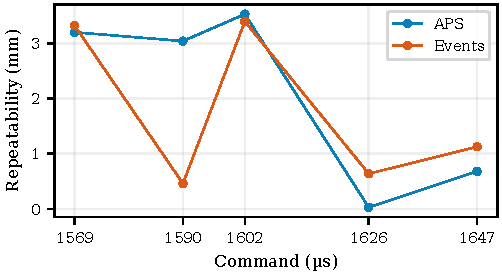
\includegraphics[width=\columnwidth]{figures/repeat_compact.pdf}
\caption{Precision on the same rows in both methods and all three trials. Lines connect tested commands only; they do not imply calibrated intermediate planes.}\label{fig:repeat}\end{figure}

An initial command-selection error used $1627\micros$, which has no fitted plane. Those three recordings are retained and excluded from depth evaluation; three separately documented $1626\micros$ captures supply the fifth fitted position. An earlier interrupted two-capture pilot is not counted as a repeat set. These exclusions are explicit in the run register and manifests.

\subsection{Unknown-filter configuration test}
The ND retry reduces the fixed-mask camera signal from $27.135\pm0.056$ digital levels ($n=2$) to $11.657\pm0.088$ ($n=3$), where uncertainty is sample SD across acquisitions (Table~\ref{tab:nd}). The ratio 0.4296 is not 43\% optical transmission (Fig.~\ref{fig:ndvisual}). Median stripe-coordinate differences of approximately $-0.94$ to $-0.96$ pixels remain relative to the first recent unfiltered control; no cause is established. No feedback-screen warnings occurred in these retry traces.

\begin{table}[!t]\caption{Fixed-command filter retry: candidate rows per acquisition with unchanged primary detectors. Integration differs between methods.}\label{tab:nd}\centering
\begin{tabular}{lcll}\toprule Condition&$n$&APS rows&Event rows\\\midrule No filter&2&78, 78&20, 18\\Unknown ND&3&62, 62, 64&0, 1, 0\\\bottomrule\end{tabular}\end{table}

APS retains more rows than the selected event pipeline here. This is a negative implementation/condition result, not a general low-light limit of event cameras. Earlier filter handling produced approximately $-2$ pixels of displacement and filter removal approximately $+14$ pixels relative to a historical baseline. Those spatially confounded attempts are retained separately. A post-pilot APS diagnostic using a longer dark reference diagnoses one frame-selection failure but does not replace the frozen primary outcomes. Only two configurations are available: no filter and one unknown filter. There is no calibrated multi-level curve or weakest-usable threshold, and no new ND depth claim.

\begin{figure}[!t]\centering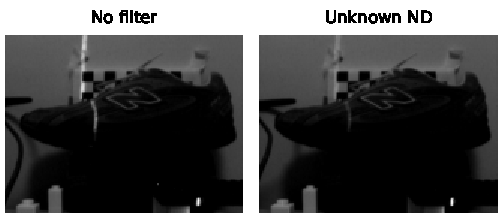
\includegraphics[width=\columnwidth]{figures/nd_APS_pair.pdf}
\caption{Fixed-$1626\micros$ filter retry at 35\,ms APS exposure. Left: recent unfiltered control; right: unknown ND. Selected median APS images use the same fixed-mask temporal-selection method and display scale. Residual stripe displacement remains; this is a configuration comparison, not calibrated transmittance or a depth result.}\label{fig:ndvisual}\end{figure}

\subsection{Static timing prediction}
Later ON markers have prediction RMS 25.74\,ms and maximum absolute residual 47.08\,ms; all OFF markers have RMS 27.00\,ms and maximum 47.55\,ms (Fig.~\ref{fig:timing}). This does not isolate clock drift from optical/event-selection effects. It does show that the implemented mapping is insufficiently validated for assigning moving laser planes to events. Static held-plane reconstruction does not require that changing-plane mapping.

\begin{figure}[!t]\centering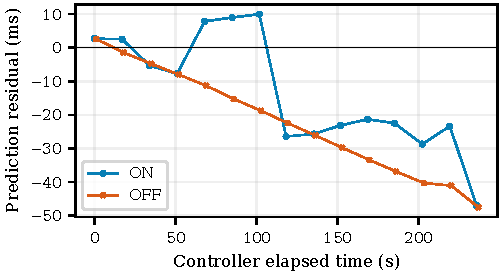
\includegraphics[width=\columnwidth]{figures/timing_compact.pdf}
\caption{Static optical-edge predictions after fitting the first five ON markers. Subsequent ON and all OFF markers are excluded from the fit. Residuals are not absolute timing uncertainty or a continuous-depth validation.}\label{fig:timing}\end{figure}

\section{Limitations, Proposal Gaps and Reproducibility}
The physical scanner, static calibration, reconstruction fallback, initial APS comparison and repeated acquisitions are demonstrated. Continuous event-based 3D reconstruction is not yet demonstrated: the camera--servo timing and moving light-plane model are insufficiently validated to assign each event a reliable plane. Further work will validate this association before the dependent speed study. Independent step/board dimensions, full 3D completeness and calibrated attenuation remain unfinished independently of the continuous-scanning blocker. They must not all be described as timing-dependent work.

\pending{G1: independent geometry}{Measured board/step dimensions, instrument resolution, datums and repeated bias/RMS/step-height error; no bias-removing test alignment.}
\pending{G2: continuous mapping}{Held-out physical timing, reset handling, motion/feedback-to-plane association and moving-stripe reconstruction.}
\pending{G3: speed}{After G2, repeated matched event/APS error and coverage versus sweep duration.}
\pending{G4: attenuation/completeness}{Measured ND levels, geometry-preserving controls, usability threshold and independently bounded 3D reference surface.}
\pending{G5: build/scope}{As-built dimensions, component/optics labels, wiring/controls, cost/parts, robustness and processing latency.}

The repository retains raw recordings, hashes, exclusions and offline scripts; new audits refuse overwrite. Eight focused synthetic checks cover analysis helpers, not physical performance. The source package supplies a verified image-coverage generator, evidence manifest and detailed pending-work ledger. \verify{marker-access repository URL, licence, unit/year/topic, stable data release and complete rebuild instructions}. Repository-only reproducibility is not yet established.

\section{Conclusion}
The team-built scanner produces real partial profiles with both APS and static event candidates. A frozen calibration supports quantitative reserved-board errors, common-mask image coverage and repeated-acquisition diagnostics. On the compared board subset, 8.07\,mm event RMS and 8.42\,mm APS RMS do not establish superiority. The filter test exposes a practical failure of the current event settings, and timing residuals motivate retaining the static fallback. The report's remaining work is explicit: independently measured geometry, continuous mapping and its dependent speed study, calibrated attenuation, true 3D completeness and reproducibility/build verification. These limitations bound the claims without discarding the measured prototype evidence.

\section*{Acknowledgments and Attribution}
Teaching staff, lab methods, cited work, OpenCV and iniVation tooling are acknowledged. OpenAI Codex assisted software, analysis, illustrations and drafting. Measurement figures use retained data; the conceptual geometry illustration is not a measurement. \verify{team contributions, attribution and final review}. Retain drafts and development materials under unit rules.

\bibliographystyle{IEEEtran}
\bibliography{references}
\end{document}
